% presentation
\documentclass{beamer}
\usetheme[height=7mm]{Rochester}
\usecolortheme{rose}

% handout

%\documentclass[handout]{beamer}
%\usepackage{pgfpages} \pgfpagesuselayout{8 on 1}[a4paper]

%\documentclass[mathserif]{article}
%\usepackage{beamerarticle}

\usepackage{amsmath}
\usepackage{comment}
\usepackage{amssymb,amsfonts}
\usepackage[T1]{fontenc}
\usepackage{lmodern}
\usepackage{tikz}
\usepackage{simpsons}
\usepackage{marvosym}
\usepackage{color}
\usepackage{multirow}
\usepackage{pgffor}
\usepackage[slide,algoruled,titlenumbered,vlined,noend,linesnumbered,]{algorithm2e}

\usefonttheme{structurebold}

\setbeamertemplate{footline}[frame number]
\setbeamertemplate{navigation symbols}{}
\setbeamerfont{smallverb}{size*={73}}
\usefonttheme[onlymath]{serif}
\setbeamertemplate{theorems}[numbered]
\newtheorem{construction}[theorem]{Construction}
\newtheorem{proposition}[theorem]{Proposition}

\AtBeginSection[] {
  \begin{frame}
    \frametitle{Content}
    \tableofcontents[currentsection]
  \end{frame}
  \addtocounter{framenumber}{-1}
}

\usetikzlibrary[shapes.arrows]
\usetikzlibrary{shapes.geometric}
\usetikzlibrary{backgrounds}
\usetikzlibrary{positioning}
\usetikzlibrary{calc}
\usetikzlibrary{intersections}
\usetikzlibrary{fadings}
\usetikzlibrary{decorations.footprints}
\usetikzlibrary{patterns}
\usetikzlibrary{shapes.callouts}
\usetikzlibrary{fit}
%handout

\providecommand{\abs}[1]{\lvert#1\rvert}

\tikzset{every picture/.style={line width=1pt,show background rectangle},background rectangle/.style={fill=blue!10,rounded corners=2ex}}

\author{Yu Zhang}
\institute{Harbin Institute of Technology}
\date[Crypto'20A]{Cryptography, Autumn, 2020}

%% presentation
\documentclass{beamer}
\usetheme[height=7mm]{Rochester}
\usecolortheme{rose}

% handout

%\documentclass[handout]{beamer}
%\usepackage{pgfpages} \pgfpagesuselayout{8 on 1}[a4paper]

%\documentclass[mathserif]{article}
%\usepackage{beamerarticle}

\usepackage{amsmath}
\usepackage{comment}
\usepackage{amssymb,amsfonts}
\usepackage[T1]{fontenc}
\usepackage{lmodern}
\usepackage{tikz}
\usepackage{simpsons}
\usepackage{marvosym}
\usepackage{color}
\usepackage{multirow}
\usepackage{pgffor}
\usepackage[slide,algoruled,titlenumbered,vlined,noend,linesnumbered,]{algorithm2e}

\usefonttheme{structurebold}

\setbeamertemplate{footline}[frame number]
\setbeamertemplate{navigation symbols}{}
\setbeamerfont{smallverb}{size*={73}}
\usefonttheme[onlymath]{serif}
\setbeamertemplate{theorems}[numbered]
\newtheorem{construction}[theorem]{Construction}
\newtheorem{proposition}[theorem]{Proposition}

\AtBeginSection[] {
  \begin{frame}
    \frametitle{Content}
    \tableofcontents[currentsection]
  \end{frame}
  \addtocounter{framenumber}{-1}
}

\usetikzlibrary[shapes.arrows]
\usetikzlibrary{shapes.geometric}
\usetikzlibrary{backgrounds}
\usetikzlibrary{positioning}
\usetikzlibrary{calc}
\usetikzlibrary{intersections}
\usetikzlibrary{fadings}
\usetikzlibrary{decorations.footprints}
\usetikzlibrary{patterns}
\usetikzlibrary{shapes.callouts}
\usetikzlibrary{fit}
%handout

\providecommand{\abs}[1]{\lvert#1\rvert}

\tikzset{every picture/.style={line width=1pt,show background rectangle},background rectangle/.style={fill=blue!10,rounded corners=2ex}}

\author{Yu Zhang}
\institute{Harbin Institute of Technology}
\date[Crypto'20A]{Cryptography, Autumn, 2020}

%\input{1introduction.tex}
%\input{2perfectlysecret.tex}
%\input{3privatekey.tex}


\title{Introduction}

\begin{document}
\maketitle
\begin{frame}
\frametitle{Outline}
\tableofcontents
\end{frame}
\section{Cryptography and Modern Cryptography}
\begin{frame}\frametitle{What is Cryptography?}
\begin{itemize}
\item \textbf{Cryptography}: from Greek \emph{krypt\'os}, ``hidden, secret''; and \emph{gr\'{a}phin}, ``writing''
\item \textbf{Cryptography}: the art of writing or solving codes.\\ (Concise oxford dictionary 2006)
\item \textbf{Codes}: a system of prearranged signals, especially used to ensure secrecy in transmitting messages. \\ (\emph{code word} in cryptography)
\item \textbf{1980s}: from Classic to Modern; from Military to Everyone
\item \textbf{Modern cryptography}: the scientific study of mathematical techniques for securing digital information, systems, and distributed computations against adversarial attacks
\end{itemize}
\end{frame}
\section{The Setting of Private-Key Encryption}
\begin{frame}\frametitle{Private-Key Encryption}
\begin{itemize}
\item \textbf{Goal}: to construct \textbf{ciphers} (encryption schemes) for providing secret communication between two parties sharing \textbf{private-key} (the symmetric-key) in advance
\item \textbf{Implicit assumption}: there is some way of initially sharing a key in a secret manner
\item \textbf{Disk encryption}: the same user at different points in time
\end{itemize}
\end{frame}
\begin{frame}\frametitle{The Syntax of Encryption}
\begin{figure}
\begin{center}
\begin{tikzpicture}
\node (sender) [minimum size=1cm] {}; \Alice{0}{0}{0.4};
\node (bart) [below of = sender, node distance = 0.7cm] {Alice};
\node (enc) [draw, right of = sender, rounded corners=1ex,node distance = 2cm] {$\mathsf{Enc}$};
\node (k1) [above of = enc, node distance = 1cm] {$k$};
\node (c) [right of = enc, node distance = 2cm] {$c$};
\node (gen) [draw, above of = c, rounded corners=1ex,node distance = 1cm] {$\mathsf{Gen}$};
\node (adv) [below of = c, node distance = 1cm, minimum size=1cm] {}; \Evil{4cm}{-1cm}{0.4};
\node (burns) [below of = adv, node distance = 0.7cm] {Adversary};
\node (dec) [draw, right of = c, rounded corners=1ex,node distance = 2cm] {$\mathsf{Dec}$};
\node (k2) [above of = dec, node distance = 1cm] {$k$};
\node (receiver) [right of = dec, node distance = 2cm, minimum size=1cm] {}; \Bob{8cm}{0}{0.4};
\node (lisa) [below of = receiver, node distance = 0.7cm] {Bob};
\draw[-latex] (sender) -- (enc) node [midway, above] {$m$};
\draw (enc) -- (c); \draw[-latex] (c) -- (dec);
\draw[-latex] (dec) -- (receiver) node [midway, above] {$m$};
\draw[-latex] (k1) -- (enc);
\draw[-latex] (gen) -- (k1);
\draw[-latex] (gen) -- (k2);								
\draw[-latex] (k2) -- (dec);		
\end{tikzpicture}
\end{center}
\end{figure}
\begin{itemize}
\item key $k \in \mathcal{K}$, plaintext (or message) $m \in \mathcal{M}$, ciphertext $c \in \mathcal{C}$
\item \textbf{Key-generation} algorithm~$k \gets \mathsf{Gen}$
\item \textbf{Encryption} algorithm~$c:= \mathsf{Enc}_k(m)$
\item \textbf{Decryption} algorithm~$m:= \mathsf{Dec}_k(c)$
\item \textbf{Encryption scheme}: $\Pi = (\mathsf{Gen}, \mathsf{Enc}, \mathsf{Dec})$
\item \textbf{Basic correctness requirement}: $\mathsf{Dec}_k(\mathsf{Enc}_k(m)) = m$
\end{itemize}
\end{frame}
\begin{frame}\frametitle{Securing Key vs Obscuring Algorithm}
\begin{itemize}
\item Easier to maintain secrecy of a short key
\item In case the key is exposed, easier for the honest parties to change the key
\item In case many pairs of people, easier to use the same algorithm, but different keys
\end{itemize}
\begin{alertblock}{Kerckhoffs's principle}
\begin{quote}
The cipher method must not be required to be secret, and it must be able to fall into the hands of the enemy without inconvenience.
\end{quote}	
\end{alertblock}
\end{frame}
\begin{frame}\frametitle{Why ``Open Cryptographic Design''}
\begin{itemize}
\item Published designs undergo public scrutiny are to be stronger
\item Better for security flaws to be revealed by ``ethical hackers''
\item Reverse engineering of the code (or leakage by industrial espionage) poses a serious threat to security
\item Enable the establishment of standards.
\end{itemize}
\end{frame}
\begin{frame}\frametitle{Attack Scenarios}	
\begin{itemize}
\item \textbf{Ciphertext-only}: the adversary just observes ciphertext
\item \textbf{Known-plaintext}: the adversary learns pairs of plaintexts/ciphertexts under the same key
\item \textbf{Chosen-plaintext}: the adversary has the ability to obtain the encryption of plaintexts of its choice
\item \textbf{Chosen-ciphertext}: the adversary has the ability to obtain the decryption of \textbf{other} ciphertexts of its choice
\item \textbf{Passive attack}: COA KPA
\begin{itemize}
\item because not all ciphertext are confidential
\end{itemize}
\item \textbf{Active attack}: CPA CCA
\begin{itemize}
\item when to encrypt/decrypt whatever an adversary wishes?
\end{itemize}
\end{itemize}	
\end{frame}
\section{Historical Ciphers and Their Cryptanalysis}
\begin{comment}
	\begin{frame}\frametitle{Why We Learn Broken Ciphers?}
	\begin{itemize}
	\item To understand the weaknesses of an ``ad-hoc'' approach
	\item To learn that ``simple'' approaches are unlikely to succeed
	\item To feel that ``we are smart enough to do some crypt-analyzing''
	\end{itemize}
	\end{frame}
\end{comment}

\begin{frame}[fragile]\frametitle{Caesar's Cipher}
\begin{quote}
If he had anything confidential to say, he wrote it in cipher, that is, by so changing the order of the letters of the alphabet, that not a word could be made out. If anyone wishes to \alert{decipher} these, and get at their meaning, he must \alert{substitute the fourth letter of the alphabet, namely D, for A}, and so with the others

\rightline{--Suetonius,``Life of Julius Caesar''}
\end{quote}
\begin{itemize}
	\item $\mathsf{Enc}(m)=m+3\mod 26$ \footnote{In fact the quote indicates that decryption involved rotating letters of the alphabet forward 3 positions, $\mathsf{Dec}(c)=c+3\mod 26$}
	\item \textbf{Weakness}: ? %\alert{What is the key?}
\end{itemize}
\begin{exampleblock}{Example}
\verb|begintheattacknow|
%\verb|EHJLQWKHDWWDFNQRZ|
\end{exampleblock}
\end{frame}
\begin{frame}[fragile]\frametitle{Shift Cipher}
\begin{itemize}
\item $\mathsf{Enc}_k(m)=m+k\mod 26$
\item $\mathsf{Dec}_k(c)=c-k\mod 26$
\item \textbf{Weakness}: ? %Fragile under \textbf{Brute-force attack} (exhaustive search)
\end{itemize}
\begin{exampleblock}{Example: Decipher the string}	
\verb|EHJLQWKHDWWDFNQRZ|
\end{exampleblock}
\begin{alertblock}{Sufficient Key Space Principle}
Any secure encryption scheme must have a key space that is not vulnerable to exhaustive search.\footnote{If the plaintext space is larger than the key space.}
\end{alertblock}
\end{frame}
\begin{frame}\frametitle{Index of Coincidence (IC) Method (to find $k$)}
\textbf{Index of Coincidence (IC)}: the probability that two randomly selected letters (pick-then-return) will be identical.

Let $p_i$ denote the probability of $i$th letter in English text.
\[I \overset{\text{def}}{=}\sum_{i=0}^{25} p_i^2 \]
\begin{exampleblock}{Example}
What's the IC of `apple'?
\end{exampleblock}

For a long English text, the IC is $\approx 0.065$.
For $j = 0, 1, \dotsc , 25$, $q_j$ is the probability of $j$th letter in the ciphertext.
\[I_j \overset{\text{def}}{=}\sum_{i=0}^{25} p_i \cdot q_{i+j}\]
\alert{Q: For shift cipher, if $j = k$, then $I_j \approx$ ?}
\end{frame}

\begin{frame}[fragile]\frametitle{Mono-Alphabetic Substitution}
\begin{itemize}
\item \textbf{Idea}: To map each character to a different one in an arbitrary manner
\item \textbf{Strength}: Key space is large $\approx 2^{88}$. \alert{Q: how to count?}
\item \textbf{Weakness}: ? %The mapping of each letter is fixed
\end{itemize}
\begin{exampleblock}{Example}
\verb|abcdefghijklmnopqrstuvwxyz|\\
\verb|XEUADNBKVMROCQFSYHWGLZIJPT|

Plaintext: \verb|tellhimaboutme|\\
Ciphertext: \verb|??????????????|
\end{exampleblock}
\end{frame}
\begin{frame}[fragile]\frametitle{Attack with Statistical Patterns}
\begin{enumerate}
\item Tabulate the frequency of letters in the ciphertext
\item Compare it to those in English text
\item Guess the most frequent letter corresponds to \verb|e|, and so on
\item Choose the plaintext that does ``make sense'' (Not trivial)
\end{enumerate}
\begin{table}
\begin{center}
\caption{Average letter frequencies for English-language text}
\begin{tabular}{|cc|cc|cc|cc|cc|} \hline
e & 12.7\% & t & 9.1\% & a & 8.2\% & o & 7.5\% & i & 7.0\%\\
n & 6.7\% & \_ & 6.4\% & s & 6.3\% & h & 6.1\% & r & 6.0\%\\
d & 4.3\% & l & 4.0\% & c & 2.8\% & u & 2.8\% & m & 2.4\%\\
w & 2.4\% & f & 2.2\% & g & 2.0\% & y & 2.0\% & p & 1.9\%\\
b & 1.5\% & v & 1.0\% & k & 0.8\% & j & 0.2\% & x & 0.2\%\\
q & 0.1\% & z & 0.1\% & & & & & &\\ \hline
\end{tabular}
\end{center}
\end{table}
\end{frame}
\begin{frame}[fragile]\frametitle{Example of Frequency Analysis (Ciphertext)}
\begin{verbatim}
LIVITCSWPIYVEWHEVSRIQMXLEYVEOIEWHRXEXIPFEMVEWHKVS
TYLXZIXLIKIIXPIJVSZEYPERRGERIMWQLMGLMXQERIWGPSRIH
MXQEREKIETXMJTPRGEVEKEITREWHEXXLEXXMZITWAWSQWXSWE
XTVEPMRXRSJGSTVRIEYVIEXCVMUIMWERGMIWXMJMGCSMWXSJO
MIQXLIVIQIVIXQSVSTWHKPEGARCSXRWIEVSWIIBXVIZMXFSJX
LIKEGAEWHEPSWYSWIWIEVXLISXLIVXLIRGEPIRQIVIIBGIIHM
WYPFLEVHEWHYPSRRFQMXLEPPXLIECCIEVEWGISJKTVWMRLIHY
SPHXLIQIMYLXSJXLIMWRIGXQEROIVFVIZEVAEKPIEWHXEAMWY
EPPXLMWYRMWXSGSWRMHIVEXMSWMGSTPHLEVHPFKPEZINTCMXI
VJSVLMRSCMWMSWVIRCIGXMWYMX
\end{verbatim}
\end{frame}
\begin{frame}[fragile]\frametitle{Example of Frequency Analysis (Analysis)}
Count and Guess, Trial and Error.
\begin{table}
\begin{center}
\caption{Analysis Steps}
\begin{tabular}{|r|l|} \hline
Ciphertext & Plaintext \\ \hline
\alert{I}   & \alert{e} \\
\alert{XLI} & \alert{the} \\
\alert{E} & \alert{a} \\
\alert{R}tate & \alert{s}tate \\
atthatt\alert{MZ}e & atthatt\alert{im}e \\
he\alert{V}e & he\alert{r}e \\
remar\alert{A} & remar\alert{k} \\ \hline
\end{tabular}
\end{center}
\end{table}
\end{frame}
\begin{frame}[fragile]\frametitle{Example of Frequency Analysis (Plaintext)}
\begin{quote}
Hereupon Legrand arose, with a grave and stately air, and brought me the beetle
from a glass case in which it was enclosed. It was a beautiful scarabaeus, and, at
that time, unknown to naturalists -- of course a great prize in a scientific point
of view. There were two round black spots near one extremity of the back, and a
long one near the other. The scales were exceedingly hard and glossy, with all the
appearance of burnished gold. The weight of the insect was very remarkable, and,
taking all things into consideration, I could hardly blame Jupiter for his opinion
respecting it.

\rightline{--Edgar Allan Poe's ``The Gold-Bug''}
\end{quote}
\end{frame}

\begin{frame}[fragile]\frametitle{Vigen\`{e}re (poly-alphabetic shift) Cipher}
\begin{itemize}
\item \textbf{Idea}: To ``smooth out'' the distribution in the ciphertext by mapping different instances of the same letter in the plaintext to different ones in the ciphertext
\item \textbf{Encryption}: $c_i=m_i+k_{[i\bmod t]}$, $t$ is the length (period) of $k$
\item \textbf{Cryptanalysis}: Need find $t$; if $t$ is known, need know whether the decryption ``makes sense'', but brute force ($26^t$) is infeasible for $t > 15$
\end{itemize}
\begin{exampleblock}{Example (Key is `cafe')}
\begin{description}[Ciphertext]
\item[Plaintext]  \verb|tellhimaboutme| \\
\item[Key]        \verb|cafecafecafeca| \\
\item[Ciphertext] \verb|??????????????| %\verb|WFRQKJSFEPAYPF|
\end{description}
\end{exampleblock}
\end{frame}
\begin{frame}[fragile]\frametitle{Kasiski's Method (to find $t$)}
\begin{itemize}
\item To identify repeated patterns of length 2 or 3
\item The distance between such appearances is a multiple of $t$
\item $t$ is the greatest common divisor of all the distances
\end{itemize}
\begin{exampleblock}{Example (Key is `beads')}
\begin{semiverbatim}
themanandthewomanretrievedtheletterfromthepostoffice
beadsbeadsbeadsbeadsbeadsbeansdeadsbeadsbeadsbeadbea
VMFQTPFOH\alert{MJJ}XSFCSSIMTNFZXFYISEIYUIKHWPQ\alert{MJJ}QSLVTGJKGF
\end{semiverbatim}
\end{exampleblock}
\end{frame}
\begin{frame}\frametitle{Index of Coincidence (IC) Method (to find $t$)}
For $\tau = 1, 2, \dotsc$, $q_i$ is the probability of $i$th letter in $c_1, c_{1+\tau}, c_{1+2\tau}, \dotsc$, IC is
\[I_\tau \overset{\text{def}}{=}\sum_{i=0}^{25} q_i^2\]
\alert{If $\tau = t$, then $I_\tau \approx ?$} ; otherwise $q_i \approx \frac{1}{26}$ and
\[I_\tau \approx \sum_{i=0}^{25} \left(\frac{1}{26}\right)^2 \approx 0.038\]
Then reuse IC method to find $k_i$.
\begin{alertblock}{Arbitrary Adversary Principle}
Security must be guaranteed for any adversary within the class of adversaries having the specified power
\end{alertblock}
\end{frame}
\begin{frame}\frametitle{Cryptanalytic Attacks (homework assignment)}
\begin{itemize}
\item Under COA, the requirement for ciphertext related to the size of the key space.  Vig\`{e}nere > mono-alphabetic sub. > shift
\item Under KPA, trivially broken.
\end{itemize}
\begin{alertblock}{Lessons learned}
\begin{itemize}
\item Sufficient key space principle
\item Designing secure cipher is a hard task
\item Complexity does not imply security (then what does?)
\item Arbitrary adversary principle
\end{itemize}
\end{alertblock}
\end{frame}
\section{The Basic Principles of Modern Cryptography}
\begin{frame}\frametitle{Three Main Principles of Modern Cryptography}
\begin{enumerate}
\item The formulation of a rigorous \textbf{definition} of security / threat model
\item When the security of a cipher relies on an unproven \textbf{assumption}, this assumption must be precisely stated and be as minimal as possible
\item Cipher should be accompanied by a rigorous \textbf{proof} of security with the above definition and the above assumption
\end{enumerate}
\end{frame}
\begin{frame}\frametitle{Why Principle 1 -- Formulation of Exact Definitions}
\begin{exampleblock}{Q: how would you formalize the security for private-key encryption?}
\begin{enumerate}
\item \emph{No adversary can find the secret key when given a ciphertext.}\\
$\mathsf{Enc}_k(m)=m$
\item \emph{No adversary can find the plaintext that corresponds to the ciphertext.}\\
$\mathsf{Enc}_k(m)=m_{0}\| \mathsf{AES}_k(m)$
\item \emph{No adversary can determine any character of the plaintext that corresponds to the ciphertext.}\\
$m=1000$, someone can learn $ 800 < m < 1200$
\item \emph{No adversary can derive any meaningful information about the plaintext from the ciphertext.}\\
Could you define so-called `meaningful'?
\end{enumerate}
\emph{\alert{Definitions of security should suffice for all potential applications.}}
\end{exampleblock}
\end{frame}
\begin{frame}\frametitle{Why Principle 1 -- How to define}
%\begin{exampleblock}{General Form}
%A cryptographic scheme for a given \textbf{task} is secure if no adversary of a specified \textbf{power} can achieve a specified \textbf{break}
%\end{exampleblock}

How To Define Security -- Lesson From Alan Turing
\begin{itemize}
\item What's computation?\footnote{Q: Any ``mathematical proof that there exist well-defined problems that computers cannot solve''? A: Halting Problem in computability theory}
\begin{enumerate}
\item A direct appeal to \textbf{intuition}
\item A \textbf{proof of the equivalence} of two definitions\\ (The new one has a greater intuitive appeal)
\item Giving \textbf{examples} solved using a definition
\end{enumerate}
\item Additional method for security: \textbf{Test of time}
\end{itemize}
\end{frame}	
\begin{frame}\frametitle{Principle 2 -- Reliance on Precise Assumptions}
Most cryptographic constructions \textbf{cannot be proven secure unconditionally}
\begin{itemize}
	\item \textbf{Why?} 
	\begin{enumerate}
		\item Validation of the assumption
		\item Comparison of schemes
		\item Facilitation of proofs of security
	\end{enumerate}
	\textbf{The construction is secure if the assumption is true.}
	\item \textbf{How?} 
	\begin{enumerate}
		\item old, so well tested
		\item simple and lower-level, so easy to study, refute \& correct
	\end{enumerate}
\end{itemize}
\end{frame}
\begin{frame}\frametitle{Principle 3 -- Rigorous Proofs of Security}
\begin{itemize}
\item \textbf{Why?} Proofs are more desirable in computer security than in other fields.
\item \textbf{The reductionist approach}: 
\begin{theorem}	Given that Assumption X is true, Construction Y is secure according to the given definition.
\end{theorem}
\begin{proof} Reduce the problem given by X to the problem of breaking Y.
\end{proof}
\item \textbf{Ad-hoc approaches}: for those who need a ``quick and dirty'' solution, or who are just simply unaware.
\end{itemize}
\end{frame}
\begin{frame}\frametitle{Summary}
\begin{itemize}
\item Cryptography secures information, transactions and computations
\item Kerckhoffs's principle \& Open cryptographic design
\item Caesar's, shift, Mono-Alphabetic sub., Vigen\`{e}re
\item Brute force, letter frequency, Kasiski's, IC
\item Sufficient key space principle
\item Arbitrary adversary principle
\item Rigorously proven security
\end{itemize}
\end{frame}
\begin{frame}\frametitle{What is cryptography? [xkcd:504]}
\begin{figure}
\begin{center}
\includegraphics[width=100mm]{pic/legal} 
\end{center}
\end{figure}
\end{frame}
\begin{frame}\frametitle{Alice, Bob  [xkcd:1323]}
Changing the names would be easier, but if you're not comfortable lying, try only making friends with people named Alice, Bob, Carol, etc.
\begin{figure}
\begin{center}
\includegraphics[width=45mm]{pic/alice-bob} 
\end{center}
\end{figure}
\end{frame}
\end{document}


%% presentation
\documentclass{beamer}
\usetheme[height=7mm]{Rochester}
\usecolortheme{rose}

% handout

%\documentclass[handout]{beamer}
%\usepackage{pgfpages} \pgfpagesuselayout{8 on 1}[a4paper]

%\documentclass[mathserif]{article}
%\usepackage{beamerarticle}

\usepackage{amsmath}
\usepackage{comment}
\usepackage{amssymb,amsfonts}
\usepackage[T1]{fontenc}
\usepackage{lmodern}
\usepackage{tikz}
\usepackage{simpsons}
\usepackage{marvosym}
\usepackage{color}
\usepackage{multirow}
\usepackage{pgffor}
\usepackage[slide,algoruled,titlenumbered,vlined,noend,linesnumbered,]{algorithm2e}

\usefonttheme{structurebold}

\setbeamertemplate{footline}[frame number]
\setbeamertemplate{navigation symbols}{}
\setbeamerfont{smallverb}{size*={73}}
\usefonttheme[onlymath]{serif}
\setbeamertemplate{theorems}[numbered]
\newtheorem{construction}[theorem]{Construction}
\newtheorem{proposition}[theorem]{Proposition}

\AtBeginSection[] {
  \begin{frame}
    \frametitle{Content}
    \tableofcontents[currentsection]
  \end{frame}
  \addtocounter{framenumber}{-1}
}

\usetikzlibrary[shapes.arrows]
\usetikzlibrary{shapes.geometric}
\usetikzlibrary{backgrounds}
\usetikzlibrary{positioning}
\usetikzlibrary{calc}
\usetikzlibrary{intersections}
\usetikzlibrary{fadings}
\usetikzlibrary{decorations.footprints}
\usetikzlibrary{patterns}
\usetikzlibrary{shapes.callouts}
\usetikzlibrary{fit}
%handout

\providecommand{\abs}[1]{\lvert#1\rvert}

\tikzset{every picture/.style={line width=1pt,show background rectangle},background rectangle/.style={fill=blue!10,rounded corners=2ex}}

\author{Yu Zhang}
\institute{Harbin Institute of Technology}
\date[Crypto'20A]{Cryptography, Autumn, 2020}

%\input{1introduction.tex}
%\input{2perfectlysecret.tex}
%\input{3privatekey.tex}


\title{Perfectly Secret Encryption}

\begin{document}
\maketitle
\begin{frame}\frametitle{Outline}
\tableofcontents
\end{frame}
\section{Definitions and Basic Properties}
\begin{frame}\frametitle{Recall The Syntax of Encryption}
\begin{figure}
\begin{center}
\begin{tikzpicture}
\node (sender) [minimum size=1cm] {}; \Alice{0}{0}{0.4};
\node (bart) [below of = sender, node distance = 0.7cm] {Alice};
\node (enc) [draw, right of = sender, rounded corners=1ex,node distance = 2cm] {$\mathsf{Enc}$};
\node (k1) [above of = enc, node distance = 1cm] {$k$};
\node (c) [right of = enc, node distance = 2cm] {$c$};
\node (gen) [draw, above of = c, rounded corners=1ex,node distance = 1cm] {$\mathsf{Gen}$};
\node (adv) [below of = c, node distance = 1cm, minimum size=1cm] {}; \Evil{4cm}{-1cm}{0.4};
\node (burns) [below of = adv, node distance = 0.7cm] {Adversary};
\node (dec) [draw, right of = c, rounded corners=1ex,node distance = 2cm] {$\mathsf{Dec}$};
\node (k2) [above of = dec, node distance = 1cm] {$k$};
\node (receiver) [right of = dec, node distance = 2cm, minimum size=1cm] {}; \Bob{8cm}{0}{0.4};
\node (lisa) [below of = receiver, node distance = 0.7cm] {Bob};
\draw[-latex] (sender) -- (enc) node [midway, above] {$m$};
\draw (enc) -- (c); \draw[-latex] (c) -- (dec);
\draw[-latex] (dec) -- (receiver) node [midway, above] {$m$};
\draw[-latex] (k1) -- (enc);
\draw[-latex] (gen) -- (k1);
\draw[-latex] (gen) -- (k2);								
\draw[-latex] (k2) -- (dec);		
\end{tikzpicture}
\end{center}
\end{figure}
\begin{itemize}
\item $k \in \mathcal{K}, m \in \mathcal{M}, c \in \mathcal{C}$.
\item $k \gets \mathsf{Gen}, c:= \mathsf{Enc}_k(m), m:= \mathsf{Dec}_k(c)$.
\item \textbf{Encryption scheme}: $\Pi = (\mathsf{Gen}, \mathsf{Enc}, \mathsf{Dec})$.
\item \textbf{Random Variable}: $K, M, C$ for key, plaintext, ciphertext.
\item \textbf{Probability}: $\Pr[K=k], \Pr[M=m], \Pr[C=c].$
\item \alert{What's the basic correctness requirement?}
\end{itemize}
\end{frame}
\begin{frame}\frametitle{Definition of `Perfect Secrecy'}
\textbf{Intuition}: An adversary knows the probability distribution over $\mathcal{M}$. $c$ should have no effect on the knowledge of the adversary; the a \emph{posteriori} likelihood that some $m$ was sent should be no different from the a \emph{priori} probability that $m$ would be sent. 
\begin{definition}
$\Pi$ over $\mathcal{M}$ is \textbf{perfectly secret} if for every probability distribution over $\mathcal{M}$, $\forall m \in \mathcal{M}$ and $\forall c \in \mathcal{C}$ for which $\Pr[C = c] > 0$:
\[ \Pr[M=m | C=c] = \Pr[M=m].\]
\end{definition}
\textbf{Simplify}: non-zero probabilities for $\forall m \in \mathcal{M}$ and $\forall c \in \mathcal{C}$.\\

\begin{exampleblock}{Is the below scheme perfectly secret?}{ For $\mathcal{M}=\mathcal{K} = \{ 0,1 \} , \mathsf{Enc}_k(m)= m \oplus k$.}\end{exampleblock}
\end{frame}

\begin{frame}\frametitle{Perfect Secrecy On One Bit}

\begin{exampleblock}{XORing one bit is perfectly secret.}
Let $\Pr[M=1] = p$ and $\Pr[M=0] = 1-p$.
Let us consider a case that $M=1$ and $C=1$.
\[ \Pr[M=1 | C=1] = \Pr[C=1 | M=1 ] \cdot \Pr[ M=1 ] / \Pr[C=1] \]
\[ = \frac{\Pr[K = 1\oplus 1] \cdot p }{ \Pr[C=1 | M=1] \cdot \Pr[M=1] + \Pr[C=1 | M=0] \cdot \Pr[M=0]} \]
\[ = \frac{1/2 \cdot p }{ 1/2 \cdot p + 1/2 \cdot (1-p)} = p = \Pr[M=1] \]
We can do the same for other cases.
\end{exampleblock}
Note that $\Pr[M=1 | C=1] \neq \Pr[M=1, C=1] = \Pr[C=1 | M=1] \cdot \Pr[M=1] = 1/2 \cdot p$.
\end{frame}

\begin{frame}\frametitle{An Equivalent Formulation}
\begin{lemma} \label{lem:ps} 
$\Pi$ over $\mathcal{M}$ is perfectly secret $\iff$ for every probability distribution over $\mathcal{M}$, $\forall m \in \mathcal{M}$ and $\forall c \in \mathcal{C}$:
\[ \Pr[C=c | M=m] = \Pr[C=c].\]
\end{lemma}
\begin{proof}
$\Leftarrow$: Multiplying both sides by $\Pr[M=m]/\Pr[C=c]$, then use Bayes' Theorem.\footnote{If $\Pr[B]\neq 0$ then $ \Pr[A|B] = \left( \Pr[A] \cdot \Pr[B|A] \right) / \Pr[B] $} \\
$\Rightarrow$: Multiplying both sides by $\Pr[C=c]/\Pr[M=m]$, then use Bayes' Theorem.
\end{proof}
\end{frame}
\begin{frame}\frametitle{Perfect Indistinguishability}
\begin{lemma}\label{lem:pi}
$\Pi$ over $\mathcal{M}$ is perfectly secret $\iff$ for every probability distribution over $\mathcal{M}$, $\forall m_0, m_1 \in \mathcal{M}$ and $\forall c \in \mathcal{C}$:
\[ \Pr[C=c | M=m_0] = \Pr[C=c | M=m_1].\]
\end{lemma}
\begin{proof}
$\Rightarrow$: By Lemma \ref{lem:ps}: $\Pr[C=c | M=m] = \Pr[C=c]$. \\
$\Leftarrow$: $p \overset{\text{def}}{=} \Pr[C=c | M=m_0]$.
\[
\begin{split}
	\Pr[C=c] &= \sum_{m \in \mathcal{M}} \Pr[C=c|M=m] \cdot \Pr[M=m] \\
	&= \sum_{m \in \mathcal{M}} p \cdot \Pr[M=m] = p = \Pr[C=c|M=m_0].
\end{split}
\]
\end{proof}
\end{frame}
\section{The One-Time Pad (Vernam's Cipher)}
\begin{frame}\frametitle{One-Time Pad (Vernam's Cipher)}
\begin{itemize}
	\item $\mathcal{M} = \mathcal{K} = \mathcal{C} = \{0,1\}^{\ell}$.
	\item $\mathsf{Gen}$ chooses a $k$ randomly with probability exactly $2^{-\ell}$.
	\item $c := \mathsf{Enc}_k(m) = k \oplus m$. 
	\item $m := \mathsf{Dec}_k(c) = k \oplus c$. 
\end{itemize}
\begin{theorem}
The one-time pad encryption scheme is perfectly-secret.
\end{theorem}
\begin{proof}
\[\begin{split} \Pr[C=c|M=m] &= \Pr[M \oplus K=c|M=m] \\
&= \Pr[m \oplus K=c] = \Pr[K = m \oplus c] = 2^{-\ell}.
\end{split}
\]
Then Lemma \ref{lem:pi}: $\Pr[C=c | M=m_0] = \Pr[C=c | M=m_1]$.
\end{proof}
\end{frame}
\section{Limitations of Perfect Secrecy}
\begin{frame}\frametitle{Limitations of OTP and Perfect Secrecy}
Key $k$ is as long as $m$, difficult to store and share $k$.
\begin{theorem}
Let $\Pi$ be perfectly-secret over $\mathcal{M}$, and let $\mathcal{K}$ be determined by $\mathsf{Gen}$. Then $|\mathcal{K}|\ge |\mathcal{M}|$. 
\end{theorem}
\begin{proof}
Assume $|\mathcal{K}| < |\mathcal{M}|$.
$\mathcal{M}(c) \overset{\text{def}}{=} \{ \hat{m} | \hat{m} = \mathsf{Dec}_k(c)\  \text{for some}\ \hat{k} \in \mathcal{K} \}$. Since for one $k$, there is at most one $m$ such that $m = \mathsf{Dec}_k(c)$, $|\mathcal{M}(c)|\le |\mathcal{K}| < |\mathcal{M}|$. So $\exists m' \notin \mathcal{M}(c)$. Then
\[ \Pr[M=m'|C=c] = 0 \neq \Pr[M = m'] \]
and so not perfectly secret.
\end{proof}
\end{frame}
\begin{frame}\frametitle{Two Time Pad: Real World Cases}
Only used once for the same key, otherwise
\[c\oplus c'=(m\oplus k)\oplus (m'\oplus k)=m\oplus m'.\]
Learn $m$ from $m\oplus m'$ due to the redundancy of language.
\begin{exampleblock}{MS-PPTP (Win NT)}
\begin{figure}
\begin{center}
\begin{tikzpicture}
\node (sender) [minimum size=1cm,label=below:Client, label=above:$k$] {}; \Alice{0}{0}{0.4};
\node (c) at ($(sender)+(4cm,0.5cm)$) {$\left[ m_1\|m_2\|m_3\right] \oplus PRG(k)$};
\node (c1) [below of = c, node distance = 1cm] {$\left[s_1\|s_2\|s_3\right] \oplus PRG(k)$};
\node (receiver) at ($(sender)+(8cm,0)$) [minimum size=1cm,label=below:Server, label=above:$k$] {}; \Bob{8cm}{0}{0.4};
\draw[-latex] (sender.east |- c) -- (c) -- (receiver.west |- c);
\draw[-latex] (receiver.west |- c1) -- (c1) -- (sender.east |- c1);
\end{tikzpicture}
\end{center}
\end{figure}
Improvement: use two keys for C-to-S and S-to-C separately.
\end{exampleblock}
\end{frame}
\section{Shannon's Theorem}
\begin{frame}\frametitle{Shannon's Theorem}
\begin{theorem}
For $|\mathcal{M}| = |\mathcal{K}| = |\mathcal{C}|$, $\Pi$ is perfectly secret $\iff$
\begin{enumerate}
\item Every $k \in \mathcal{K}$ is chosen with probability $1/|\mathcal{K}|$ by $\mathsf{Gen}$.
\item $\forall m \in \mathcal{M}$ and $\forall c \in \mathcal{C}$, $\exists$ unique $k \in \mathcal{K}$: $c := \mathsf{Enc}_k(m)$.
\end{enumerate}
\end{theorem}
\begin{proof}
$\Leftarrow$: $\Pr[C=c|M=m]=1/|\mathcal{K}|$, use Lemma \ref{lem:pi}. \\
$\Rightarrow (2)$: At least one $k$, otherwise $\Pr[C=c|M=m]=0$; \\
at most one $k$, because $\{\mathsf{Enc}_k(m)\}_{k\in \mathcal{K}} = \mathcal{C}$ and $|\mathcal{K}| = |\mathcal{C}|$.\\
$\Rightarrow (1)$: $k_i$ is such that $\mathsf{Enc}_{k_i}(m_i)=c$.
\[ \begin{split}
\Pr[M = m_i] &= \Pr[M=m_i|C=c] \\
             &= \left( \Pr[C =c|M=m_i] \cdot \Pr[M = m_i] \right) / \Pr[C=c] \\
 &= \left( \Pr[K=k_i] \cdot \Pr[M = m_i] \right) / \Pr[C=c],
\end{split}
\]
so $\Pr[K=k_i] = \Pr[C = c] = 1/|\mathcal{K}|$.
\end{proof}
\end{frame}

\begin{frame}\frametitle{Application of Shannon's Theorem}
\begin{exampleblock}{Is the below scheme perfectly secret?}
Let $\mathcal{M} = \mathcal{C} = \mathcal{K} = \{ 0, 1, 2,\dots , 255 \} $\\
$\mathsf{Enc}_k(m) = m  + k \mod 256$\\
$\mathsf{Dec}_k(c) = c - k \mod 256$
\end{exampleblock}
\end{frame}
\section{Eavesdropping Indistinguishability}
\begin{frame}\frametitle{Eavesdropping Indistinguishability Experiment}
$\mathsf{PrivK}^{\mathsf{eav}}_{\mathcal{A},\Pi}$ denote a \textbf{priv}ate-\textbf{k}ey encryption experiment for a given $\Pi$ over $\mathcal{M}$ and an \textbf{eav}esdropping adversary $\mathcal{A}$.
\begin{enumerate}
	\item $\mathcal{A}$ outputs a pair of messages $m_0, m_1 \in \mathcal{M}$.
	\item $k \gets \mathsf{Gen}$, a random bit $b \gets \{0,1\}$ is chosen. Then $c \gets \mathsf{Enc}_k(m_b)$ is given to $\mathcal{A}$.
	\item $\mathcal{A}$ outputs a bit $b'$
	\item If $b' = b$, $\mathcal{A}$ succeeded $\mathsf{PrivK}^{\mathsf{eav}}_{\mathcal{A},\Pi}=1$, otherwise 0.
\end{enumerate}
\begin{figure}
\begin{center}
\begin{tikzpicture}
%\node (A) at (0,0) {\Homer};
%\node (B) [right of = A, node distance = 4cm] {\Left\Burns};
\node (A) at (0,0) [minimum size=1cm] {}; \Charlie{0}{0}{0.4};
\node (B) [right of = A, node distance = 4cm, minimum size=1cm] {}; \Evil{4cm}{0}{0.4};
\node (1a) [below of=A, node distance=1cm] {};
\node (1b) [below of=B, node distance=1cm] {$m_0, m_1$};
\draw[-latex] (1b) -- (1a) node [midway,above] {};
\node (2a) [below of=1a, node distance=0.5cm] {Gen $b, k$};
\node (2b) [below of=1b, node distance=0.5cm] {};
%\draw[-latex] (2b) -- (2a) node [midway,above] {};
%\node (3a) [below of=2a, node distance=0.5cm] {};
%\node (3b) [below of=2b, node distance=0.5cm] {};
\node (4a) [below of=2a, node distance=0.5cm] {$\mathsf{Enc}_k(m_b)$};
\node (4b) [below of=2b, node distance=0.5cm] {};
\draw[-latex] (4a) -- (4b) node [midway,above] {};
\node (5a) [below of=4a, node distance=0.5cm] {};
\node (5b) [below of=4b, node distance=0.5cm] {$b'$};
\draw[-latex] (5b) -- (5a) node [midway,above] {};
\node (6a) [below of=5a, node distance=0.5cm] {};
\node (6b) [below of=5b, node distance=0.5cm] {};
\node (result) [right of = 6a, node distance = 2cm] {Win if $b = b'$};
\end{tikzpicture}

\end{center}
\end{figure}
\end{frame}
\begin{frame}\frametitle{Adversarial Indistinguishability}
\begin{definition}
$\Pi$ over $\mathcal{M}$ is \textbf{perfectly secret} if for every $\mathcal{A}$ it holds that
\[ \Pr[\mathsf{PrivK}^{\mathsf{eav}}_{\mathcal{A},\Pi}=1] = \frac{1}{2}.\]
\end{definition}
\begin{exampleblock}{Which in the below schemes are perfectly secret?}
\begin{itemize}
\item $\mathsf{Enc}_{k,k'}(m)= \mathsf{OTP}_k(m) \| \mathsf{OTP}_{k'}(m)$
\item $\mathsf{Enc}_{k}(m)= reverse(\mathsf{OTP}_k(m))$
\item $\mathsf{Enc}_{k}(m)= \mathsf{OTP}_k(m) \| k$
%To break semantic security, an attacker would read the secret key from the challenge ciphertext and use it to decrypt the challenge ciphertext. Basically, any ciphertext reveals the secret key.
\item $\mathsf{Enc}_{k}(m)= \mathsf{OTP}_k(m) \| \mathsf{OTP}_k(m) $
\item $\mathsf{Enc}_{k}(m)= \mathsf{OTP}_{0^{n}}(m)$
%To break semantic security, an attacker would ask for the encryption of $0^n$ and $1^n$ and can easily distinguish EXP(0) from EXP(1) because it knows the secret key, namely 0n.
\item $\mathsf{Enc}_{k}(m)= \mathsf{OTP}_k(m) \| LSB(m)$
%To break semantic security, an attacker would ask for the encryption of $0^n$ and $0^{n-1}1$ and can distinguish EXP(0) from EXP(1).
\end{itemize}
\end{exampleblock}
\end{frame}

\begin{frame}\frametitle{Summary}
\begin{itemize}
\item Perfect secrecy $=$ Perfect indistinguishability $=$ Adversarial indistinguishability
\item Perfect secrecy is attainable. The One-Time Pad (Vernam's cipher)
\item Shannon's theorem
\end{itemize}	
\end{frame}
\end{document}

%\input{3privatekey.tex}


\title{More on Public-Key Cryptography}

\begin{document}
\maketitle
\begin{frame}
\frametitle{Outline}
\tableofcontents
\end{frame}

\section{Primes and Factoring}
\begin{frame}\frametitle{Integer Factorization/Factoring}
\begin{quote}
``The problem of distinguishing prime numbers from composite numbers and of resolving the later into their prime factors is known to be one of the most important and useful in arithmetic.'' -- Gauss (1805)
\end{quote}

The ``hardest'' numbers to factor seem to be those having only large prime factors.
\begin{itemize}
\item The best-known algorithm is the \textbf{general number field sieve} [Pollard] with time $\mathcal{O}(\exp(n^{1/3}\cdot(\log n)^{2/3}))$.
\item RSA Factoring Challenge: RSA-768 (232 digits)
\begin{itemize}
\item Two years on hundreds of machines (2.2GHz/2GB, 1500 years)
\item Factoring a 1024-bit integer: about 1000 times harder.
\end{itemize}
\end{itemize}
\end{frame}
\begin{frame}\frametitle{Generating Random Primes}
\begin{algorithm}[H]
\SetKwInOut{Input}{input}
\SetKwInOut{Output}{output}
\SetKw{KwB}{break}
\SetKw{KwH}{halt}
\DontPrintSemicolon
\caption{Generating a random prime}
\Input{Length $n$; parameter $t$}
\Output{A random $n$-bit prime}
\BlankLine
\For{$i = 1$ \KwTo $t$}{
  $p' \gets \{0,1\}^{n-1}$\;
  $p := 1\| p'$\;
  \lIf{$p$ is prime}{\Return $p$}\;
}
\Return fail
\end{algorithm}
To show its efficiency, we need understand two issues:
\begin{itemize}
\item the probability that a randomly-selected $n$-bit integer is prime.
\item how to efficiently test whether a given integer $p$ is prime.
\end{itemize}
\end{frame}
\begin{frame}\frametitle{The Distribution of Prime}
\begin{theorem}[Prime number theorem]
$\exists$ a constant $c$ such that, $\forall n>1$, a randomly selected $n$-bit number is prime with probability at least $c/n$.
\end{theorem}
The probability that a prime is \emph{not} chosen in $t = n^2/c$ iterations is
\[ \left( 1-\frac{c}{n} \right)^t = \left( \left( 1-\frac{c}{n} \right)^{n/c} \right)^n \le \left( e^{-1} \right)^n = e^{-n}.
\]
The algorithm will fail with a negligible probability.
\end{frame}
\begin{frame}\frametitle{Testing Primality}
\begin{itemize}
\item \textbf{Trial division}: Divide $N$ by $a=2,3,\dotsc,\sqrt{N}.$
\item \textbf{Probabilistic algorithm for approximately computing}:
\begin{itemize}
\item Atlantic City algorithm with two-sided error. 
\item Monte Carlo algorithm with one-sided error.
\item Las Vegas algorithm with zero-sided error.
\end{itemize}
\item \textbf{Fermat primality test}: $a^{N-1} \equiv 1 \pmod N$.
\item $a$ is a \textbf{witness} that $N$ is composite if $a^{N-1} \not \equiv 1 \pmod N$.
\item $a$ is a \textbf{liar} if $N$ is composite and $a^{N-1} \equiv 1 \pmod N$.
\item \textbf{Carmichael numbers}: composite numbers without witnesses.
\end{itemize}
\begin{theorem}
If $\exists$ a witness, then at least half the elements of $\mathbb{Z}_N^*$ are witnesses.
\end{theorem}
\end{frame}
\begin{frame}\frametitle{The Miller-Rabin Primality Test}
$N-1=2^ru$, $u$ is odd. $a \in \mathbb{Z}^*_N$ is a \textbf{strong witness} if
\begin{enumerate}
\item $a^u \neq \pm 1$, and
\item $a^{2^iu} \neq -1$ for $i\in\{1,\dotsc,r-1\}$.
\end{enumerate}
\begin{lemma}
$x \in \mathbb{Z}^*$ is a \textbf{square root of 1 modulo} $N$ if $x^2 \equiv 1 \pmod N$. If $N$ is an odd prime then the only $x$ are $[\pm 1 \bmod N]$.
\end{lemma}
\begin{theorem}
$N$ is an odd, composite number that is not a prime power. Then at least half the elements of $\mathbb{Z}^*_N$ are strong witnesses.
\end{theorem}
\begin{theorem}
If $N$ is prime, then the Miller-Rabin test always outputs ``prime''. If $N$ is composite, then the algorithm outputs ``prime'' with probability at most $2^{-t}\;$\footnote{Actually, it is at most $4^{-t}$.}.
\end{theorem}
\end{frame}
\begin{frame}\frametitle{Describing The Algorithm}
\begin{algorithm}[H]
\SetKwInOut{Input}{input}
\SetKwInOut{Output}{output}
\SetKw{KwC}{compute}
\SetKw{KwL}{LOOP}
\DontPrintSemicolon
\caption{The Miller-Rabin primality test}
\Input{Integer $N>2$ and parameter $t$}
\Output{A decision as to wether $N$ is prime or composite}
\BlankLine

\lIf{$N$ is a perfect power}{\Return ``composite''}
\KwC $r\ge 1$ and $u$ odd such that $N-1 = 2^ru$\;
\KwL: \For{$s = 1$ \KwTo $t$}{
  $a \gets \{2,\dotsc,N-2\}$\;
  $x = a^u \bmod N$\;
  \lIf{$x = \pm 1$}{do next \KwL}
  \For{$i = 1$ \KwTo $r$} {
    $x = x^2 \bmod N$\;
    \lIf{$x = -1 $}{do next \KwL}
%    \lIf{$x = 1 $}{\Return ``composite''}\;
  }
  \Return ``composite''\;
}
\Return ``prime''
\end{algorithm}
\end{frame}
\begin{frame}\frametitle{Examples of Primality Tests}
\begin{exampleblock}{Liars in Fermat primality test}
$2^{340} \equiv 1 \pmod {341}$,  but $341 = 11\cdot 31$.\\  
$5^{560} \equiv 1 \pmod {561}$,  but $561 = 3\cdot 11\cdot 17$.\\
Carmichael numbers $< 10000$: \\  
561,  1105,  1729,  2465,  2821,  6601,  8911.
\end{exampleblock}
\begin{exampleblock}{Examples of Miller-Rabin test}
Carmichael number $1729=7\cdot 13\cdot 19$. \\$1729-1 = 1728 = 2^6\cdot 27$. So $r = 6, u = 27$. $a=671$.
\begin{align*}
671^{27} &\equiv 1084 \pmod {1729} \\
671^{27\cdot 2} &\equiv 1065 \pmod {1729}\\
671^{27\cdot 2^2} &\equiv 1 \pmod {1729}\\
\end{align*}

\end{exampleblock}
\end{frame}
\begin{frame}\frametitle{Algorithms for Factoring}
\begin{itemize}
\item \textbf{Factoring} $N=pq$. $p,q$ are of the same length $n$.
\item \textbf{Trial division}: $\mathcal{O}(\sqrt{N}\cdot \mathsf{polylog}(N))$.
\item \textbf{Pollard's $p-1$} method: effective when $p-1$ has ``small'' prime factors.
\item \textbf{Pollard's rho} method: $\mathcal{O}(N^{1/4}\cdot \mathsf{polylog}(N))$.
\item \textbf{Quadratic sieve} algorithm [Carl Pomerance]: sub-exponential time $\mathcal{O}(\exp(\sqrt{n\cdot \log n}))$.
\item The best-known algorithm is the \textbf{general number field sieve} [Pollard] with time $\mathcal{O}(\exp(n^{1/3}\cdot(\log n)^{2/3}))$.
\end{itemize}
\end{frame}
\begin{frame}\frametitle{Pollard's $p-1$ Method}
\textbf{Idea}: Fermat's little theorem: $y = x^{(p-1)\cdot k} \equiv 1 \pmod p$. Then $(y-1) \equiv 0 \pmod p$ and $p \mid (y-1)$. So $p = \gcd(y-1,N)$. To make the exponent a large multiple of $(p-1)$:
\[ M = lcm(\{ i | i \le B \}) = \prod_{\text{prime}\;i \le B}i^{\lfloor \log_iB \rfloor}.\]
If $p-1$ has only ``small'' factors, then the bound $B$ will be small.
\begin{algorithm}[H]
\SetKwInOut{Input}{input}
\SetKwInOut{Output}{output}
\SetKw{KwC}{compute}
\SetKw{KwL}{LOOP}
\DontPrintSemicolon
\caption{Pollard's $p-1$ algorithm for factoring}
\Input{Integer $N$}
\Output{A non-trivial factor of $N$}
\BlankLine

$x \gets \mathbb{Z}^*_N$\;
$y := [x^M \bmod N]$\;
$p := \gcd(y-1,N)$\;
\lIf{$p \notin \{1,N\}$}{\Return $p$}
\end{algorithm}
\end{frame}
\begin{frame}\frametitle{Pollard's Rho ($\rho$) Method}
\textbf{Idea}: Using the improved birthday attack\footnote{Floyd's cycle-finding algorithm (the ``tortoise and the hare'' algorithm).} to find $x,x'$ such that $x \neq x' \land x \equiv x' \pmod p$. Then $p \mid (x-x')$, $p = \gcd(x-x',N)$.
$F(x) = x^2+b$, where $b \not \equiv 0,-2 \pmod N$.
\begin{algorithm}[H]
\SetKwInOut{Input}{input}
\SetKwInOut{Output}{output}
\SetKw{KwC}{compute}
\SetKw{KwL}{LOOP}
\DontPrintSemicolon
\caption{Pollard's rho algorithm for factoring}
\Input{Integer $N$}
\Output{A non-trivial factor of $N$}
\BlankLine

$x_0 \gets \mathbb{Z}^*_N$\;
\For{$i=1$ \KwTo $2^{n/2}$}{
$x_i := [F(x_{i-1}) \bmod N]$\;
$x_{2i} := [F(F(x_{2i-2})) \bmod N]$\;
$p := \gcd(x_{2i}-x_i,N)$\;
\lIf{$p \notin \{1,N\}$}{\Return $p$}
}
\end{algorithm}
\end{frame}
\begin{frame}\frametitle{Proof of Pollard's $\rho$ Method}
\begin{lemma}
Let $x_1,\dotsc$ be a sequence with $x_m \equiv F(x_{m-1}) \pmod N$. $F$ satisfies that $x \equiv x' \pmod N \implies F(x) \equiv F(x') \pmod N$. If $x_I \equiv x_J\pmod p$ with $I < J$, then $\exists$ $i < J$ such that $x_{i} \equiv x_{2i} \pmod p$.
\end{lemma}
\begin{figure}
\begin{center}
\input{tikz/birthdayattack}
\end{center}
\end{figure}
\begin{proof}
See the proof of improved birthday attack.
\end{proof}
According to the lemma of birthday problem, given a sequence of length $O(N^{1/4})$, find such pair with probability $1/4$.
\end{frame}
\begin{frame}\frametitle{Example of Pollard's $p-1$ and $\rho$ methods}
\begin{exampleblock}{Factorizing $N=5917$ with Pollard's $p-1$ method}
Choose $B=5$, $M=lcm(1,2,3,4,5)=60$.\\
For $x=2$, $y \equiv x^M \equiv 2^{60} \equiv 3417 \pmod{5917}$.\\
$p = gcd(y-1,N) = \gcd(3416,5917) = 61$.
\end{exampleblock}
\begin{exampleblock}{Factorizing $N=8051$ with Pollard's $\rho$ method}
$f(x) = x^2+1$, $x_0=2$.\\
\begin{center}
\begin{tabular}{|c|c|c|c|} \hline
$i$  & $x_i$ & $x_{2i}$ & $\gcd(x_{2i}-x_i,N)$ \\ \hline
1 & 5 & 26 & 1 \\
2 & 26 & 7474 & 1 \\
3 & 677 & 871 & 97 \\ \hline
\end{tabular}	
\end{center}
\end{exampleblock}
\end{frame}
\begin{frame}\frametitle{The Quadratic Sieve Algorithm}
\textbf{Idea}: Find $x,y$ with $x^2 \equiv y^2 \pmod N$ and $x \not \equiv \pm y \pmod N$. $x^2-y^2 \equiv 0 \pmod N\implies (x+y)(x-y) \equiv 0 \pmod N$.\\
$\gcd(x+y,N)$ and $\gcd(x-y,N)$ will give $p$.\\
\textbf{Finding congruence of squares}: \\
%Find $x_i^2 \equiv y_i \pmod N$ for $i=1,2,\dotsc,r$ and $y_1y_2\cdots y_r = c^2$. \\
%$(x_1x_2\cdots x_r)^2 \equiv y_1y_2\cdots y_r = c^2 \pmod N$.\\
\begin{enumerate}
\item Choose a factor base $B = \{p_1,\dotsc,p_k\}$ of prime numbers. 
\item Use `\textbf{sieve theory}' to find $\ell = k+1$ distinct $x_1,\dotsc,x_\ell$ for which $[x_i^2 \bmod N]$ decompose into the elements of $B$: $x_i^2 \equiv \prod^k_{j=1} p_j^{e_j} \pmod N$.
\item Write $x_i^2$ as an exponent vector $\langle e_{i,1},\dotsc,e_{i,k}\rangle \pmod 2$.
\item Find the addition of vectors = the zero vector $\pmod 2$.\\
$X=\{x_{\ell_1},\dotsc,x_{\ell_n}\}$. $\forall i$, $E_i = \sum_{j=1}^ne_{\ell_j,i} \equiv 0 \pmod 2$.
\item Find a pair: $x = \prod_{i=1}^nx_{\ell_i} \not \equiv y=\prod_{i=1}^kp_i^{E_i/2} \pmod N$.  
\end{enumerate}
\end{frame}
\begin{frame}\frametitle{Example of Quadratic Sieve Algorithm}
\begin{exampleblock}{Factorizing $N=377753$ with quadratic sieve algorithm}
$B = \{2,13,17,23,29\}$.
\begin{align*}
620^2 &\equiv 17^2\cdot 23 \pmod N\\
621^2 &\equiv 2^4\cdot 17\cdot 29 \pmod N\\
645^2 &\equiv 2^7\cdot 13\cdot 23 \pmod N\\
655^2 &\equiv 2^3\cdot 13\cdot 17\cdot 29 \pmod N
\end{align*}
\[ [620\cdot 621\cdot 645\cdot 655 \bmod N]^2 \equiv [2^7\cdot 13\cdot 17^2\cdot 23\cdot 29\bmod N]^2 \]
\[ \implies 127194^2 \equiv 45335^2 \pmod N,\]
Computing $\gcd(127194-45335,377753)=751$.
\end{exampleblock}
\end{frame}
\section{Discrete Logarithm Algorithms}
\begin{frame}\frametitle{Overview of Discrete Logarithm Algorithms}
\begin{itemize}
\item Given a generator $g \in \mathbb{G}$ and $y \in \langle g \rangle$, find $x$ such that $g^x=y$.
\item \textbf{Brute force}: $\mathcal{O}(q)$, $q = \mathsf{ord}(g)$ is the order of $\langle g\rangle$.
\item \textbf{Baby-step/giant-step} method [Shanks]: $\mathcal{O}(\sqrt{q}\cdot \mathsf{polylog}(q))$.
\item \textbf{Pohlig-Hellman} algorithm: when $q$ has small factors.
\item \textbf{Index calculus} method: $\mathcal{O}(\exp{(\sqrt{n\cdot \log n})})$.
\item The best-known algorithm is the \textbf{general number field sieve} with time $\mathcal{O}(\exp(n^{1/3}\cdot(\log n)^{2/3}))$.
\item Elliptic curve groups vs. $\mathbb{Z}_p^*$: more efficient for the honest parties, but that are equally hard for an adversary to break.\\ (Both 1024-bit $\mathbb{Z}_p^*$ and 132-bit elliptic curve need $2^{66}$ steps.)
\end{itemize}
\end{frame}
\begin{frame}\frametitle{The Baby-Step/Giant-Step Algorithm}
\begin{figure}
\begin{center}
\input{tikz/baby-giant}
\end{center}
\end{figure}
\begin{algorithm}[H]
\SetKwInOut{Input}{input}
\SetKwInOut{Output}{output}
\SetKw{KwC}{compute}
\SetKw{KwS}{sort}
\DontPrintSemicolon
\caption{The baby-step/giant-step algorithm}
\Input{$g \in \mathbb{G}$ and $y \in \langle g \rangle$; $q=\mathsf{ord}(g)$ ($t := \lfloor \sqrt{q}\rfloor$)}
\Output{$\log_g y$}
\BlankLine

\lFor{$i = 0$ \KwTo $\lfloor q/t \rfloor$}{\KwC $g_i := g^{i\cdot t}$ \tcc*[f]{giant steps}}
\KwS the pairs $(i,g_i)$ by $g_i$\;
\For{$i = 0$ \KwTo $t$}{
\KwC $y_i := y\cdot g^i$ \tcc*[f]{baby steps}\;
\lIf{$y_i = g_k$ for some $k$}{\Return $[kt-i \bmod q]$}
}
\end{algorithm}
The time complexity is $\mathcal{O}(\sqrt{q}\cdot \mathsf{polylog}(q))$.
\end{frame}
\begin{frame}\frametitle{Example of Baby-Step/Giant-Step Algorithm}
\begin{exampleblock}{In $\mathbb{Z}^*_{29}$, $q=28$, $g=2$, $y=17$.}
$t=5$, compute the giant steps:
\[2^0=1,\; 2^5=3,\; 2^{10}=9,\; 2^{15}=27,\; 2^{20}=23,\; 2^{25}=11. \]
compute the baby steps:
\[17\cdot 2^0=17,\; 17\cdot 2^1=5,\; 17\cdot 2^2=10,\]
\[ 17\cdot 2^3=20,\; 17\cdot 2^4=11,\; 17\cdot 2^5=22.\]
$2^{25}=11=17\cdot 2^4$. So $\log_2 17=25-4=21$.
\end{exampleblock}

\end{frame}
\begin{frame}\frametitle{The Pohlig-Hellman Algorithm}
\textbf{Idea}: when $q$ is known and has small factors, reduces the discrete logarithm instance to multiple instances in groups of smaller order.
\newline

According to CRT: If $q=\prod^k_{i=1}q_i$ and $\forall i\neq j, \gcd(q_i,q_j)=1$, then
\[ \mathbb{Z}_q \simeq \mathbb{Z}_{q_1} \times \cdots \times \mathbb{Z}_{q_k}\; \text{and}\; \mathbb{Z}^*_q \simeq \mathbb{Z}^*_{q_1} \times \cdots \times \mathbb{Z}^*_{q_k} \]
\[(g_i)^x\overset{\text{def}}{=} \left( g^{q/q_i} \right)^x = (g^x)^{q/q_i} = y^{q/q_i}\; \text{for}\; i=1,\dotsc,k.\]
We have $k$ instances in $k$ smaller groups, $\mathsf{ord}(g_i) = q_i.\;$ \footnote{If $p \mid q$, then $\mathsf{ord}(g^p)=q/p$.}\\
Use any other algorithm to solve $\log_{g_i}  (y^{q/q_i})$.\\
Answers are $\{x_i\}^k_{i=1}$ for which $g_i^{x_i} \equiv y^{q/q_i} \equiv g_i^x$. \\
$\forall i,\;x \equiv x_i \pmod{q_i}$. $x \bmod q$ is uniquely determined (CRT). \\
The time complexity is $\mathcal{O}(\max_i\{\sqrt{q_i}\}\cdot \mathsf{polylog}(q))$.
\end{frame}
\begin{frame}\frametitle{Example of Pohlig-Hellman Algorithm}
\begin{exampleblock}{In $\mathbb{Z}^*_{31}$, $q=30=5\cdot 3 \cdot 2$, $g=3$, $y=26=g^x$.}
\begin{alignat*}{3}
(g^{30/5})^x & = y^{30/5} & \implies (3^{6})^x\;\, & = 26^{6} & \implies 16^x & \equiv 1 \\
(g^{30/3})^x & = y^{30/3} & \implies (3^{10})^x & = 26^{10} & \implies 25^x & \equiv 5 \\
(g^{30/2})^x & = y^{30/2} & \implies (3^{15})^x & = 26^{15} & \implies 30^x & \equiv 30 
\end{alignat*}
\[ x \equiv 0 \pmod 5,\; x \equiv 2 \pmod 3, x \equiv 1 \pmod 2, \]
so $x \equiv 5 \pmod{30}$.
\end{exampleblock}
\end{frame}
\begin{frame}\frametitle{The Index Calculus Method}
\textbf{Idea}: find a relatively small factor base and build a system of $\ell$ linear equations related to $g$; find a linear equation related to $y$; solve $\ell+1$ linear equations to give $\log_g y$.
\begin{enumerate}
\item for $\mathbb{Z}^*_p$, choose a base $B = \{p_1,\dotsc,p_k\}$ of prime numbers. 
\item find $\ell \ge k$ distinct $x_1,\dotsc,x_\ell$ for which $[g^{x_i} \bmod p]$ decompose into the elements of $B$: $g^{x_i} \equiv \prod^k_{j=1} p_j^{e_j} \pmod p$.
\item $\ell$ equations: $x_i = \sum^k_{j=1}e_{i,j}\cdot \log_g(p_{j}) \pmod{p-1}$.
\item find $x^*$ for which $[g^{x^*}\cdot y \bmod p]$ can be factored.
\item new equation: $x^* + \log_gy = \sum^k_{j=1}e^*_{j}\cdot \log_g(p_j) \pmod{p-1}$.
\item Use linear algebra to solve equations and give $\log_gy$.  
\end{enumerate}
The time complexity is identical to that of the quadratic sieve.
\end{frame}
\begin{frame}\frametitle{Example of Index Calculus Method}
\begin{exampleblock}{$p=101$, $g=3$ and $y=87$. $B=\{2,5,13\}$.}
$3^{10} \equiv 65 \pmod {101}$ and $65 = 5\cdot 13$. Similarly, $3^{12} \equiv 80  = 2^4 \cdot 5 \pmod {101}$ and $3^{14} \equiv 13 \pmod {101}$. The linear equations:
\begin{align*}
x_1 = 10 &\equiv \log_3 5 + \log_3 13 \pmod{100}\\
x_2 = 12 &\equiv 4\cdot \log_3 2 + \log_3 5 \pmod{100}\\
x_3 = 14 &\equiv \log_3 13 \pmod{100}.
\end{align*}
We also have $x^*=5$, $3^5\cdot 87 \equiv 32 \equiv 2^5 \pmod{101}$, or
\[5+\log_3 87 \equiv 5\cdot \log_3 2 \pmod{100}.\]
Adding the 2nd and 3rd equations and subtracting the 1st, we derive $4\cdot \log_3 2 \equiv 16 \pmod{100}$. So $\log_3 2$ is 4, 29, 54, or 79. Trying all shows that $\log_3 2 = 29$. The last equation gives $\log_3 87 = 40$.
\end{exampleblock}
\end{frame}
\section{More Public-key Schemes}
\begin{frame}\frametitle{Additional Public-key Schemes}
\begin{itemize}
\item \textbf{Goldwasser-Micali} based on deciding quadratic residuosity problem. (first scheme proven to be CPA-secure)
\item \textbf{Rabin}: based on the computing square root problem. (security equivalent to the hardness of factoring)
\item \textbf{Paillier}: based on the decisional composite residuosity problem. (efficient and homomorphic)
\item \textbf{Elliptic curve}: forms a cyclic group with DH problem (efficient).
\end{itemize}
\end{frame}
\begin{frame}\frametitle{Quadratic Residues Modulo a Prime}
\begin{itemize}
\item $y \in \mathbb{G}$ is a \textbf{quadratic residue (qr)} if $\exists x \in \mathbb{G}$ with $x^2 = y$. Otherwise, $y$ is a \textbf{quadratic non-residue (qnr)}.
\item In an abelian group, the set of qr forms a subgroup.
\item In $\mathbb{Z}_p^*$, $p> 2$ is prime, every qr has two square roots.
\item The set of qr/qnr is $\mathcal{QR}_p$/$\mathcal{QNR}_p$,
$\abs{\mathcal{QR}_p}= \abs{\mathcal{QNR}_p} = \frac{p-1}{2}$.
\item $\mathcal{J}_p(x)$ is \textbf{Jacobi symbol} of $x$ modulo $p$:

\[
  \mathcal{J}_p(x) \overset{\mathsf{def}}{=} \left\{ 
  \begin{array}{l l}
    +1 & \quad \text{if $x$ is a qr}\\
    -1 & \quad \text{if $x$ is not a qr}\\
  \end{array} \right .
\]
\item $\mathcal{J}_p(x) = x ^{\frac{p-1}{2}} \bmod p$.
\item $\mathcal{J}_p(xy) = \mathcal{J}_p(x)\cdot \mathcal{J}_p(y)$.
\end{itemize}
\end{frame}
\begin{frame}\frametitle{Quadratic Residues Modulo a Composite}
\begin{itemize}
\item $N = pq$, $p,q$ distinct primes, in Chinese Remainder Theorem: 
$x \in \mathbb{Z}_N^*$ with $ x \leftrightarrow (x_p,x_q) = ([x \bmod p], [x \bmod q])$.
\item $x$ is a qr mod $N$ $\iff$ $x_p$/$x_q$ are qr mod $p$/$q$.
\item $x$ is a qr mod $N$ $\iff \mathcal{J}_p(x) = \mathcal{J}_q(x) = +1$.
\item Qr $x$ has 4 roots: $(\pm x_p, \pm x_q)$, so $\frac{\abs{\mathcal{QR}_N}}{\abs{Z_N^*}} = \frac{\abs{\mathcal{QR}_p}\abs{\mathcal{QR}_q}}{\abs{Z_N^*}}=\frac{1}{4}$.
\item $\mathcal{J}_N(x) \overset{\mathsf{def}}{=} \mathcal{J}_p(x) \cdot \mathcal{J}_q(x)$. $\mathcal{J}_N(xy) = \mathcal{J}_N(x)\cdot \mathcal{J}_N(y)$.
\item $\mathcal{QNR}_N^{+1}(x) \overset{\mathsf{def}}{=} \{ x | x \text{ is qnr, but } \mathcal{J}_N(x) = +1\}$.
%\item $[xy \bmod N] \in \mathcal{QR}_N \text{ if } x,y \in \mathcal{QR}_N \text { or } \mathcal{QNR}_N^{+1}$.
%\item $[xy \bmod N] \in \mathcal{QNR}_N^{+1} \text{ if } x \in \mathcal{QR}_N \text{ and } y \in \mathcal{QNR}_N^{+1}$.
\end{itemize}
\begin{figure}
\begin{center}
\input{tikz/qr-qnr.tex}
\end{center}
\end{figure}
\end{frame}
\begin{frame}\frametitle{Goldwasser-Micali Scheme}
\begin{itemize}
\item \textbf{Deciding quadratic residuosity (DQR)} of $x$, where $x$ is randomly chosen from $\mathcal{J}_N^{+1}$ ($\mathcal{QR}_N$ and $\mathcal{QNR}_N^{+1}$).
\item For DQR, no solution is better than factoring $N$.
\end{itemize}
\begin{construction}
\begin{itemize}
\item $\mathsf{Gen}$: $(N,p,q)$, $z \gets \mathcal{QNR}_N^{+1}$. $pk = \left<N,z\right>$ and $sk=\left<p,q\right>$.
\item $\mathsf{Enc}$: $m\in \{0,1\}$, $x\gets \mathbb{Z}_N^*$, output $c := [z^m\cdot x^2 \bmod N]$.
\item $\mathsf{Dec}$: If $c$ is a qr, output $0$; otherwise $1$.
\end{itemize}
\end{construction}
Goldwasser-Micali scheme is CPA-secure if DQR problem is hard.
\end{frame}
\begin{frame}\frametitle{Computing Square Roots mod a Prime}
\begin{algorithm}[H]
\SetKwInOut{Input}{input}
\SetKwInOut{Output}{output}
\SetKw{KwC}{compute}
\SetKw{KwS}{sort}
\SetKw{KwCA}{case}
\DontPrintSemicolon
\caption{computing square root of a prime}
\Input{Prime $p$; quadratic residue $a \in \mathbb{Z}^*_p$}
\Output{A square root of $a$}
\BlankLine

\KwCA $p=3 \bmod 4$:
\Return $[a^{\frac{p+1}{4}} \bmod p]$\;
\KwCA $p=1 \bmod 4$:
let $b$ be a qnr modulo $p$\;
\KwC $l$ and $m$ odd with $2^\ell\cdot m = \frac{p-1}{2}$\;
$r := 2^\ell$, $r' := 0$\;
\For{$i = \ell$ \KwTo $1$}{ $r := r/2$, $r' := r'/2$\tcc*[f]{maintain $a^r\cdot b^{r'}=1 \bmod p$}\;
\lIf{$a^r\cdot b^{r'} = -1 \bmod p$}{$r' := r' + 2^\ell \cdot m$}
}
\tcc{now $r=m$, $r'$ is even, and $a^r\cdot b^{r'}=1 \bmod p$}
\Return $\left[ a^{\frac{r+1}{2}}\cdot b^{\frac{r'}{2}} \bmod p\right]$\;
\end{algorithm}
\end{frame}
\begin{frame}\frametitle{Rabin Scheme}
\begin{itemize}
\item \textbf{Computing square roots (CSR)} of qr mod $N$ is \textbf{proven to be hard} if factoring $N$ is hard.
\item $N=pq$ is a \textbf{Blum integer} if $p \ne q$ and $p \equiv q \equiv 3 \bmod 4$.
\item $\mathcal{QR}$ for Blum integer can form TDP.
\end{itemize}
\begin{construction}
\begin{itemize}
\item $\mathsf{Gen}$: Blum integer $N=pq$, $pk = N$ and $sk=\left<p,q\right>$.
\item $\mathsf{Enc}$: $m\in \{0,1\}$, $x\gets \mathcal{QR}_N$, output $c := \left< [x^2 \bmod N],\mathsf{lsb}(x)\oplus m\right>$.
\item $\mathsf{Dec}$: Input $\left<c,c'\right>$. $x=c^{1/2}$, output $\mathsf{lsb}(x)\oplus c'$.
\end{itemize}
\end{construction}
Rabin scheme is CPA-secure if factoring problem is hard.
\end{frame}
\begin{frame}\frametitle{Paillier Scheme}
\begin{itemize}
\item $\mathbb{Z}_N\times \mathbb{Z}_N^* \simeq \mathbb{Z}_{N^2}^*$ with $f(a,b)=[(1+N)^a\cdot b^N \bmod N^2]$.
\item $\mathsf{Res}(N^2)$ is the set of $N$th residue mod $N^2$: $\{(0,b) | b \in \mathbb{Z}_N^*\}$.
\item \textbf{Decisional composite residuosity (DCR)} problem is to distinguish a random element of $\mathbb{Z}_{N^2}^*$ from one of $\mathsf{Res}(N^2)$. 
\end{itemize}
\begin{construction}
\begin{itemize}
\item $\mathsf{Gen}$: $(N,p,q)$, $pk = N$ and $sk=\left<N,\phi(N)\right>$.
\item $\mathsf{Enc}$: $m\in \mathbb{Z}_N$, $r\gets \mathbb{Z}_N^*$, output $c := [(1+N)^m\cdot r^N \bmod N^2]$.
\item $\mathsf{Dec}$: output $\left[ \frac{[c^{\phi(N)} \bmod N^2]-1}{N}\cdot \phi(N)^{-1} \bmod N\right]$.
\end{itemize}
\end{construction}
$c^{\phi(N)} \bmod N^2 \leftrightarrow (m,r)^{\phi(N)} = (m\cdot {\phi(N)}, r^{\phi(N)}).$ \\
Paillier scheme is CPA-secure if DCR problem is hard.
\end{frame}
\begin{frame}\frametitle{Homomorphic Encryption}
\begin{itemize}
\item \textbf{Homomorphic Encryption} with $\circ$: $\mathsf{Dec}_{sk}(c_1\circ c_2)=m_1\circ m_2$.
\item Elgamal encryption is homomorphic with $\times$: $\left<g^{y_1},h^{y_1}\cdot m_1\right>\cdot \left<g^{y_2},h^{y_2}\cdot m_2\right> = \left<g^{y_1+y_2},h^{y_1+y_2}\cdot m_1m_2\right>$
\item Paillier scheme is homomorphic with $+$: $\mathsf{Enc}_N(m_1) \cdot \mathsf{Enc}_N(m_2) = \mathsf{Enc}_N([m_1+m_2 \bmod N])$.
\item \textbf{Application}: voting without learning any individual votes.
\[c_i := [(1+N)^{v_i}\cdot r^N \bmod N^2], v_i \in \{0,1\}\]
\[c^* := [\Pi_{i} c_i \bmod N^2], v^* = \Sigma_{i} v_i \]
\item First \textbf{Fully} homomorphic with $\times$ and $+$ by Craig Gentry in 2009.
\end{itemize}
\end{frame}
\begin{frame}\frametitle{Elliptic Curve Groups}
\textbf{Elliptic curve group}: points with ``addition'' operation.\\
Any \textbf{elliptic curve} is a plane algebraic curve:
\[ y^2 \equiv x^3 + Ax + B \pmod p\]
where $A,B \in \mathbb{Z}_p$ are constants with $4A^3 + 27B^2\not \equiv 0 \pmod p$.
$\hat{E}(\mathbb{Z}_p)$ is the set of pairs $(x,y) \in \mathbb{Z}_p \times \mathbb{Z}_p$:
\[ \hat{E}(\mathbb{Z}_p) \overset{\text{def}}{=} \{(x,y) \mid x,y\in \mathbb{Z}_p \land y^2 \equiv x^3 + Ax + B \pmod p \}\]
$E(\mathbb{Z}_p) \overset{\text{def}}{=} \hat{E}(\mathbb{Z}_p)\cup \{\mathcal{O}\}$, $\mathcal{O}$ is identity, ``\textbf{point at infinity}''.
\end{frame}
\begin{frame}\frametitle{``Addition'' on Points of Elliptic Curves}
\begin{columns}
\begin{column}{5cm}
\begin{figure}
\begin{center}
%\begin{tikzpicture}[scale=0.7]

\newcommand*{\ShowIntersection}{
\fill 
    [name intersections={of=ec1 and l1, name=i, total=\t}] 
    [red, opacity=1, every node/.style={above left, black, opacity=1}] 
    \foreach \s in {1,...,\t}{(i-\s) circle (2pt)
        node [above left] {\s}};
}

    \begin{axis}[
            xmin=-4,
            xmax=4,
            ymin=-4,
            ymax=4,
            %grid=both,
            %grid style={line width=.1pt, draw=gray!10},
            %major grid style={line width=.2pt,draw=gray!50},
            %xlabel={$x$},
            %ylabel={$y$},
            %scale only axis,
            xtick=\empty, ytick=\empty,
            axis lines=middle,
            domain=-2.279018:2.6,      
            samples=101,
            smooth,   
            clip=false,
            % use same unit vectors on the axis
            %axis equal image=true,
        ]
    \addplot[name path global=ec1, blue] {sqrt(x^3-3*x+5)};
    \addplot[name path global=ec2, blue] {-sqrt(x^3-3*x+5)};
    \addplot[name path global=l1, domain=-3:3, red] {0.8*x+1.3};
    \addplot[name path global=v1, orange] coordinates {(2.23,-3.8) (2.23,3.8)};
    %\addplot[name path global=t1, brown] coordinates {(-1,2.7) (2.23,3.1)};
    \addplot[name path global=t2, purple,domain=-3:3] {0.1238*x+2.824};
    \addplot[mark=*] coordinates {(2.23,-3.1)} node [below left] {$-P_3$}; 
    \addplot[mark=*] coordinates {(-1.05,2.65)} node [above left] {$P_4$}; 
    %\ShowIntersection;

\fill 
    [name intersections={of=ec1 and l1, by={p2, p3}}] 
    [black, opacity=1]
    (p2) circle (2pt) node [above] {$P_2$}
    (p3) circle (2pt) node [above left] {$P_3$};

\fill 
    [name intersections={of=ec2 and l1, by={p1}}] 
    [opacity=1] 
    (p1) circle (2pt) node [left] {$P_1$};

    %\coordinate[label={10:$P$}] (P) at (axis cs:-1,2.64);
\end{axis}

    %\draw[red,name path=curve2] (-2,-1) -- (2,2);

%    \fill [name intersections={of=ec1 and curve2, by={a,b}}]
%     (a) circle (2pt) node [above left] {$P_3$}
%     (b) circle (2pt) node [above] {$P_2$}
     %(c) circle (2pt) node [left] {$P_1$};

% \draw[dotted,gray,name path=curve3] (1.43,-2) -- (1.43,2);
% \draw[-latex,gray] (-2,0) -- (2,0);
% \draw[-latex,gray] (0,-2) -- (0,2);
% %\draw[blue,name path=curve1] plot[smooth] file {tikz/outfile};
% \draw[red,name path=curve2] (-2,-1) -- (2,2);

% \fill [name intersections={of=curve1 and curve2, by={a,b,c}}]
% (a) circle (2pt) node [above left] {$P_3$}
% (b) circle (2pt) node [above] {$P_2$}
% (c) circle (2pt) node [left] {$P_1$};
% \fill [name intersections={of=curve1 and curve3, by={a,d}}]
% (d) circle (2pt) node [left] {$-P_3$};
% %\fill [name intersections={of=curve1 and curve4, by={a,b}}]
% %(b) circle (2pt) node [left] {$P_4$};
% \node (eq) at (-1,-1.7) {\small $y^2=x^3-x+1$};
% \draw[green] (-2,0.94) node [black,above] {$P_4$} -- (a);
% \draw[fill] (-0.7,1.18) circle (1.5pt);
\end{tikzpicture}
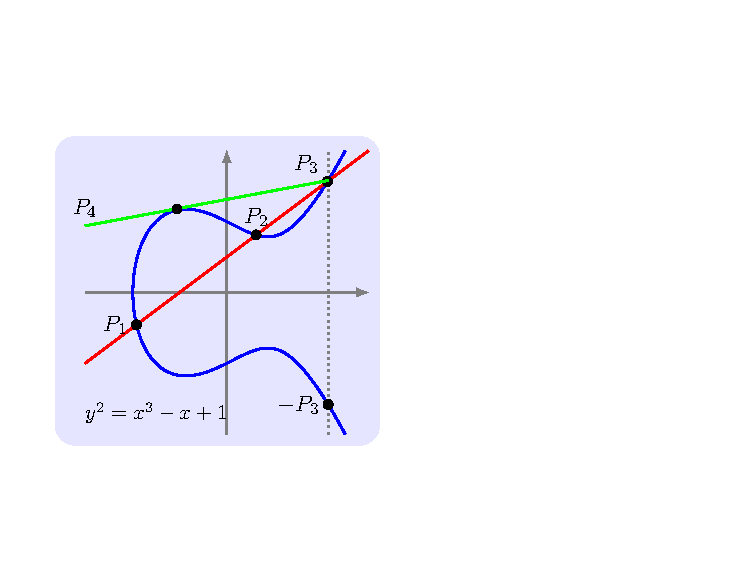
\includegraphics[width=50mm]{pic/ecc.pdf} 
\end{center}
\end{figure}
\end{column}
\begin{column}{5cm}
Every line intersects the curve in 3 points:
\begin{itemize}
\item count twice if tangent.
\item count $\mathcal{O}$ at the vertical infinity of $y$-axis.
\end{itemize}
``\textbf{Addition}'' on points:
\begin{itemize}
\item $P+\mathcal{O} = \mathcal{O} + P = P$.
\item If $P_1, P_2, P_3$ are co-linear, then $P_1 + P_2 + P_3 = \mathcal{O}$.
\end{itemize}
$-P=(x,-y)$\\
$P_1 + P_2 = -P_3$\\
$2P_4=-P_3$\\
$dP = P + (d-1)P$
\end{column}
\end{columns}
\[sk = (P,d); pk = (P,Q=dP)\]
\end{frame}
\begin{frame}\frametitle{Key Size Comparison}
\begin{center}
\textbf{Key lengths} (in bits) with comparable security
\newline

\begin{tabular}{|c|c|c|} \hline
Symmetric & RSA/DH & ECC \\ \hline	
56 & 512 & 112 \\
80 & 1024 & 160 \\
112 & 2048 & 224 \\
128 & 3072 & 256 \\
192 & 7680 & 384 \\
256 & 15360 & 521 \\ \hline	
\end{tabular}	
\end{center}
\end{frame}
\end{document}
